\documentclass{beamer}
\usetheme{CambridgeUS}

% Đặt màu cho các block
\setbeamercolor{block title}{bg=red!80!black, fg=white}
\setbeamercolor{block body}{bg=red!10, fg=black}
%%%%%%%%%%%%%%%%%%%%%%%%%%%%%%%%%%%%%%%%%%%%%%%%%%%%%%%
% vietnam
\usepackage[utf8]{vietnam}
% Dùng để thêm hình ảnh
\usepackage{graphicx}
% Dùng để di chuyển các tham chiếu
\usepackage{hyperref}
% Dùng để tạo văn bản ngẫu nhiên
\usepackage{lipsum}
% \usepackage{xcolor}
%
\usepackage{tikz}
%%%%%%%%%%%%%%%%%%%%%%%%%%%%%%%%%%%%%%%%%%%%%%%%%%%%%%%
\AtBeginSection[]
{
\begin{frame}<beamer>
\frametitle{Nội dung}

\tableofcontents[
currentsection,
subsectionstyle=hide/hide,
subsubsectionstyle=hide/hide
]

\end{frame}
}
%%%%%%%%%%%%%%%%%%%%%%%%%%%%%%%%%%%%%%%%%%%%%%%%%%%%%%%
\AtBeginSubsection[]
{
\begin{frame}<beamer>
\frametitle{Nội dung}

\tableofcontents[
currentsection,
currentsubsection,
subsectionstyle=show/shaded/hide,
%
% subsubsectionstyle=hide/hide
subsubsectionstyle=show/show/shaded/hide
]

\end{frame}
}
%%%%%%%%%%%%%%%%%%%%%%%%%%%%%%%%%%%%%%%%%%%%%%%%%%%%%%%
\title[{\makebox[.15\paperwidth]{Human Resources Management}}]{Chủ đề: Human Resources Management}
\author[Nhóm 22]{Nhóm 22}
\date[Data Warehouse \& BI]{\today}
%%%%%%%%%%%%%%%%%%%%%%%%%%%%%%%%%%%%%%%%%%%%%%%%%%%%%%%
\begin{document}
%%%%%%%%%%%%%%%%%%%%%%%%%%%%%%%%%%%%%%%%%%%%%%%%%%%%%%%
% \begin{frame}
% \begin{tikzpicture}[remember picture, overlay]
% \node[anchor=center, inner sep=0pt] at (current page.center) {
\includegraphics[width=\paperwidth, height=\paperheight]{pictures/HUST2.jpeg}};
% \fill[white, opacity=0.8] (current page.south west) rectangle (current page.north east);
% \end{tikzpicture}
% \titlepage
% \end{frame}
%%%%%%%%%%%%%%%%%%%%%%%%%%%%%%%%%%%%%%%%%%%%%%%%%%%%%%%
% \begin{frame}{Danh sách thành viên}
% \begin{block}{Nhóm 22}
% \centering
% \begin{tabular} {|l|c|}
% \hline
% Họ và tên & MSSV \\
% \hline
% Nguyễn Việt Anh & 20216796 \\
% Phùng Quốc Đạt & 20216813 \\
% Vũ Văn Nghĩa & 20206205 \\
% Mai Thị Tuyết Nhung & 20216866 \\
% \hline
% \end{tabular}
% \end{block}
% \end{frame}
%! %%%%%%%%%%%%%%%%%%%%%%%%%%%%%%%%%%%%%%%%%%%%%%%%%%%%%%
%! %%%%%%%%%%%%%%%%%%%%%%%%%%%%%%%%%%%%%%%%%%%%%%%%%%%%%%
%! %%%%%%%%%%%%%%%%%%%%%%%%%%%%%%%%%%%%%%%%%%%%%%%%%%%%%%
%! %%%%%%%%%%%%%%%%%%%%%%%%%%%%%%%%%%%%%%%%%%%%%%%%%%%%%%
%! %%%%%%%%%%%%%%%%%%%%%%%%%%%%%%%%%%%%%%%%%%%%%%%%%%%%%%
\section{Khảo sát}
% \subsection{Tổng quan về quản lý nhân sự}
% \subsubsection{Giới thiệu về quản lý nhân sự}
% \begin{frame}{Giới thiệu về quản lý nhân sự}
% \begin{columns}
% \begin{column}{0.4\textwidth}
% 
\includegraphics[width=\textwidth]{pictures/Giới thiệu về HRM.png}
% \end{column}
% \begin{column}{0.6\textwidth}
% \begin{itemize}
% \item HRM là gì?
% \item HRM là gì?
% \item \dots
% % ![alt text](image-22.png)
% % https://talentbold.com/hrm-la-gi-tat-tan-tat-ve-human-resource-management-939-ns
% % https://en.wikipedia.org/wiki/Human_resource_management
% % <!-- Video nhóm 6 -->
% % <!-- Video download -->
% \end{itemize}
% \end{column}
% \end{columns}
% \end{frame}
%%%%%%%%%%%%%%%%%%%%%%%%%%%%%%%%%%%%%%%%%%%%%%%%%%%%%%%
% \subsubsection{Vòng đời nhân sự}
% % ![alt text](image-16.png)
% % <!-- Video download -->
% % 12345678
% \begin{frame}{Vòng đời nhân sự}
% \begin{figure}[H]
% \centering
% 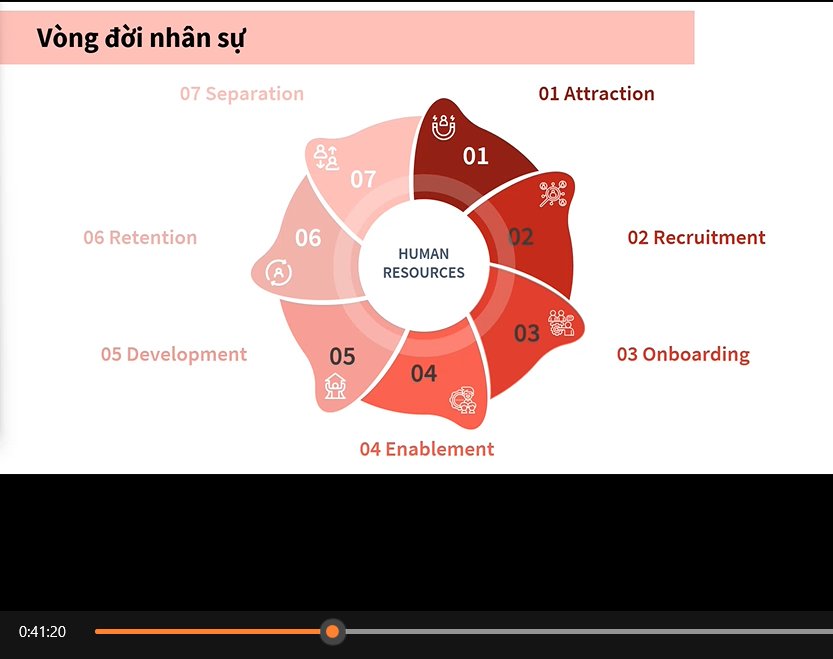
\includegraphics[scale = 0.3]{pictures/Vòng đời nhân sự.png}
% \end{figure}
% \end{frame}
%%%%%%%%%%%%%%%%%%%%%%%%%%%%%%%%%%%%%%%%%%%%%%%%%%%%%%%
% \subsection{Quy trình nghiệp vụ}
% \subsubsection{Business Model Canvas}
% % https://som.edu.vn/mo-hinh-business-model-canvas-la-gi
% \begin{frame}{Business Model Canvas}
% \begin{figure}[H]
% \centering
% 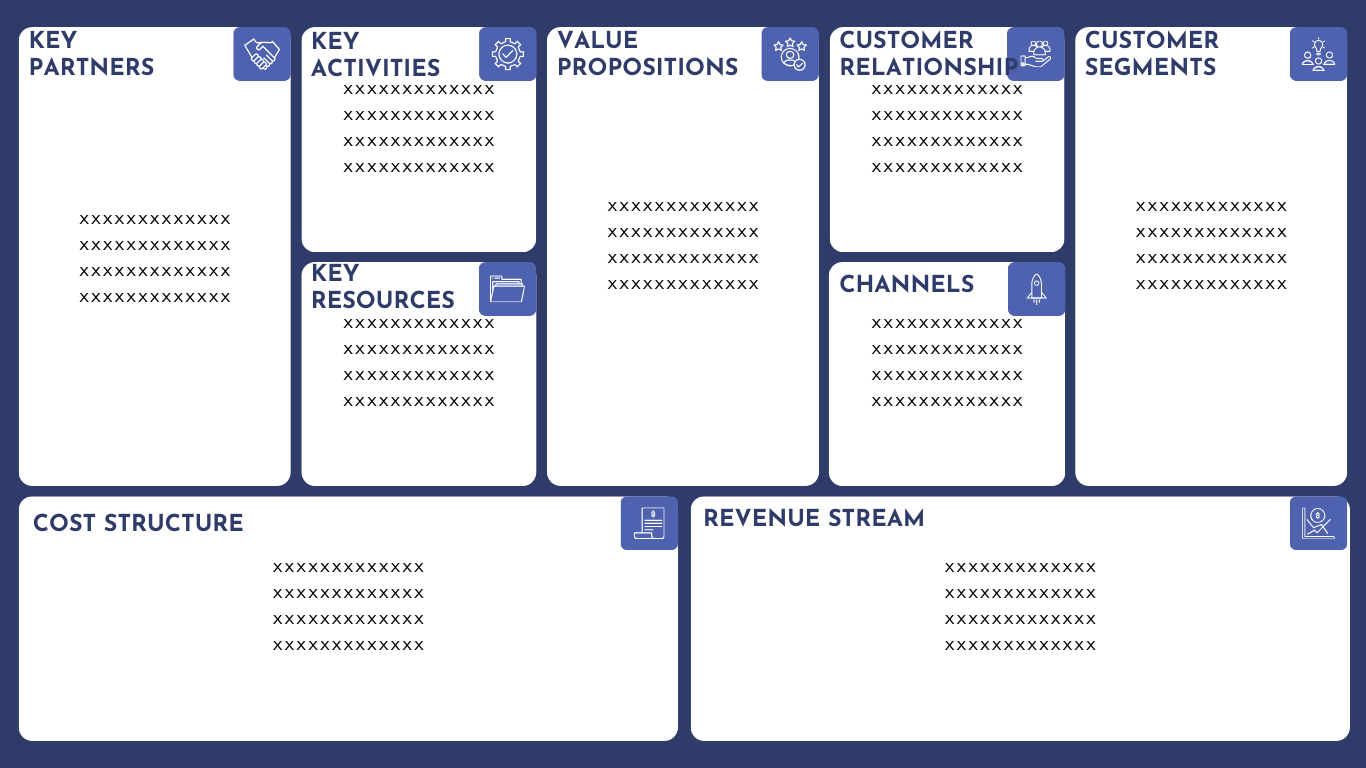
\includegraphics[scale = 0.3]{pictures/Business Model Canvas.png}
% % https://www.canva.com/design/DAGDrYFhMzE/9A5DeAlx2KgP-Aa-wmN-Nw/edit?utm_content=DAGDrYFhMzE&utm_campaign=designshare&utm_medium=link2&utm_source=sharebutton
% \end{figure}
% \end{frame}
%%%%%%%%%%%%%%%%%%%%%%%%%%%%%%%%%%%%%%%%%%%%%%%%%%%%%%%
% \subsubsection{Mô tả quy trình nghiệp vụ}
% % <!-- có đánh dấu hệ thống phân tích ở những giai đoạn nào của quy trình -->
% \begin{frame}{Mô tả quy trình nghiệp vụ}
% \begin{figure}[H]
% \centering
% 
\includegraphics[scale = 0.3]{pictures/black.png}
% % <!-- Bảng UML -->
% \end{figure}
% \end{frame}
%%%%%%%%%%%%%%%%%%%%%%%%%%%%%%%%%%%%%%%%%%%%%%%%%%%%%%%
% \subsubsection{Cây nghiệp vụ}
% % Cây nghiệp vụ là ntn???
% \begin{frame}{Cây nghiệp vụ}
% \begin{figure}[H]
% \centering
% 
\includegraphics[scale = 0.3]{pictures/black.png}
% \end{figure}
% \end{frame}
%%%%%%%%%%%%%%%%%%%%%%%%%%%%%%%%%%%%%%%%%%%%%%%%%%%%%%%
% \subsection{Yêu cầu phân tích}
% \subsubsection{Yêu cầu phân tích}
% % <!-- *) Trình bày theo các chủ điểm cần phân tích -->
% % <!-- *) Các chủ điểm này cần quan tâm theo các khía cạnh gì -->
% % ![alt text](image-3.png)
% % Phân tích xxxx theo xxxx
% % INPUT
% % OUTPUT
% % ![alt text](image-23.png)
% % ![alt text](image-24.png)
% % ![alt text](image-25.png)
% % ![alt text](image-26.png)
% \begin{frame}{Yêu cầu phân tích}
% \begin{figure}[H]
% \centering
% 
\includegraphics[scale = 0.3]{pictures/black.png}
% \end{figure}
% \end{frame}
%%%%%%%%%%%%%%%%%%%%%%%%%%%%%%%%%%%%%%%%%%%%%%%%%%%%%%%
% \subsubsection{Cây chủ điểm Vũ Văn Nghĩa ?????}
% % Cây chủ điểm Vũ Văn Nghĩa ????? là ntn???
% \begin{frame}{Cây chủ điểm Vũ Văn Nghĩa ?????}
% \begin{figure}[H]
% \centering
% 
\includegraphics[scale = 0.3]{pictures/black.png}
% \end{figure}
% \end{frame}
%%%%%%%%%%%%%%%%%%%%%%%%%%%%%%%%%%%%%%%%%%%%%%%%%%%%%%%
% \subsubsection{Cây yêu cầu phân tích}
% % Cây yêu cầu phân tích là ntn???
% \begin{frame}{Cây yêu cầu phân tích}
% \begin{figure}[H]
% \centering
% 
\includegraphics[scale = 0.3]{pictures/black.png}
% \end{figure}
% \end{frame}
%%%%%%%%%%%%%%%%%%%%%%%%%%%%%%%%%%%%%%%%%%%%%%%%%%%%%%%
% \subsubsection{Cây phân tích dashboard}
% % Cây phân tích dashboard là ntn???
% \begin{frame}{Cây phân tích dashboard}
% \begin{figure}[H]
% \centering
% 
\includegraphics[scale = 0.3]{pictures/black.png}
% \end{figure}
% \end{frame}
%%%%%%%%%%%%%%%%%%%%%%%%%%%%%%%%%%%%%%%%%%%%%%%%%%%%%%%
% \subsection{Hệ thống dữ liệu}
% \subsubsection{Quy mô của dữ liệu}
% % % ...
% % % số lượng bản ghi
% \begin{frame}{Quy mô của dữ liệu}
% \begin{columns}
% \begin{column}{0.6\textwidth}
% \begin{itemize}
% \item Tên bộ dữ liệu: xxxxxxxxxxx
% \item Mô tả: Bộ dữ liệu về xxxx từ năm 2222 đến năm 2222
% \item Nguồn dữ liệu: kaggle/xxxxxxxxx
% \item Kích thước bộ dữ liệu: xxxxx > 100 MB
% \item Số dòng: xxxxx
% \item Số cột: xxxxx
% \item Gồm xxxx files:
% \begin{itemize}
% \item xxxxxxxxxxx
% \item xxxxxxxxxxx
% \item xxxxxxxxxxx
% \item xxxxxxxxxxx
% \end{itemize}
% \end{itemize}
% \end{column}
% \begin{column}{0.4\textwidth}
% 
\includegraphics[width=\textwidth]{pictures/black.png}
% \end{column}
% \end{columns}
% \end{frame}
%%%%%%%%%%%%%%%%%%%%%%%%%%%%%%%%%%%%%%%%%%%%%%%%%%%%%%%
% \subsubsection{Mô tả thông tin dữ liệu}
% % ![alt text](image-28.png)
% % <!-- Mô tả các trường dữ liệu -->
% % Bảng xxx, dòng xxx để làm gì
% % Có thể kẻ bảng Cột xxxx: làm gì...
% \begin{frame}{}
% \begin{block}{Mô tả thông tin dữ liệu}
% \centering
% \begin{tabular} {|l|c|}
% \hline
% Tên cột & Mô tả \\
% \hline
% xxxxxxxxxxx & xxxxxxxxxxx \\
% xxxxxxxxxxx & xxxxxxxxxxx \\
% xxxxxxxxxxx & xxxxxxxxxxx \\
% xxxxxxxxxxx & xxxxxxxxxxx \\
% xxxxxxxxxxx & xxxxxxxxxxx \\
% \hline
% \end{tabular}
% \end{block}
% \end{frame}
%%%%%%%%%%%%%%%%%%%%%%%%%%%%%%%%%%%%%%%%%%%%%%%%%%%%%%%
% \subsubsection{Tần suất cập nhật dữ liệu}
% % hình ảnh (dạng biểu đồ theo thời gian)
% % => nhận xét tăng giảm....
% \begin{frame}{Tần suất cập nhật dữ liệu}
% \begin{figure}[H]
% \centering
% 
\includegraphics[scale = 0.2]{pictures/black.png}
% \end{figure}
% \begin{block}{Nhận xét}
% xxxxxxxxx
% \end{block}
% \end{frame}
%%%%%%%%%%%%%%%%%%%%%%%%%%%%%%%%%%%%%%%%%%%%%%%%%%%%%%%
% \subsubsection{Dự báo tần suất cập nhật dữ liệu mới}
% % AI
% \begin{frame}{Dự báo tần suất cập nhật dữ liệu mới}
% \begin{figure}[H]
% \centering
% 
\includegraphics[scale = 0.2]{pictures/black.png}
% \end{figure}
% \begin{block}{Nhận xét}
% xxxxxxxxx
% \end{block}
% \end{frame}
%%%%%%%%%%%%%%%%%%%%%%%%%%%%%%%%%%%%%%%%%%%%%%%%%%%%%%%
% \subsubsection{Phân loại dữ liệu Data Taxonomy}
% % Phân loại dữ liệu Data Taxonomy là ntn???
% \begin{frame}{Phân loại dữ liệu Data Taxonomy}
% \begin{figure}[H]
% \centering
% 
\includegraphics[scale = 0.3]{pictures/black.png}
% \end{figure}
% \end{frame}
%%%%%%%%%%%%%%%%%%%%%%%%%%%%%%%%%%%%%%%%%%%%%%%%%%%%%%%
% \subsubsection{Luồng dữ liệu}
% % Luồng dữ liệu là ntn???
% % <!-- Bảng UML -->
% \begin{frame}{Luồng dữ liệu}
% \begin{figure}[H]
% \centering
% 
\includegraphics[scale = 0.3]{pictures/black.png}
% \end{figure}
% \end{frame}
%%%%%%%%%%%%%%%%%%%%%%%%%%%%%%%%%%%%%%%%%%%%%%%%%%%%%%%
% \subsubsection{Mô hình ERD hệ thống OLTP}
% % Mô hình ERD hệ thống OLTP là ntn???
% <!-- *) Trên OLTP có gạch chân các trường dữ liệu và ghi chú mapping tương ứng khi chuyển sang OLAP -->
% xanh lá + Màu
% \begin{frame}{Mô hình ERD hệ thống OLTP}
% \begin{figure}[H]
% \centering
% 
\includegraphics[scale = 0.3]{pictures/black.png}
% \end{figure}
% \end{frame}
%%%%%%%%%%%%%%%%%%%%%%%%%%%%%%%%%%%%%%%%%%%%%%%%%%%%%%%
%! %%%%%%%%%%%%%%%%%%%%%%%%%%%%%%%%%%%%%%%%%%%%%%%%%%%%%%
%! %%%%%%%%%%%%%%%%%%%%%%%%%%%%%%%%%%%%%%%%%%%%%%%%%%%%%%
%! %%%%%%%%%%%%%%%%%%%%%%%%%%%%%%%%%%%%%%%%%%%%%%%%%%%%%%
%! %%%%%%%%%%%%%%%%%%%%%%%%%%%%%%%%%%%%%%%%%%%%%%%%%%%%%%
%! %%%%%%%%%%%%%%%%%%%%%%%%%%%%%%%%%%%%%%%%%%%%%%%%%%%%%%
\section{Phân tích và Thiết kế}
%%%%%%%%%%%%%%%%%%%%%%%%%%%%%%%%%%%%%%%%%%%%%%%%%%%%%%%
\subsection{Kiến trúc hệ thống phân tích dữ liệu}
\begin{frame}{Kiến trúc hệ thống phân tích dữ liệu}

\begin{columns}

\begin{column}{0.24\textwidth}

\includegraphics[width=\textwidth]{pictures/DATA SOURCES.png}
% https://www.canva.com/design/DAGDr5h1pEE/gsFg-GK1Y2-pzTf8nBDexA/edit?utm_content=DAGDr5h1pEE&utm_campaign=designshare&utm_medium=link2&utm_source=sharebutton
\end{column}

\begin{column}{0.24\textwidth}
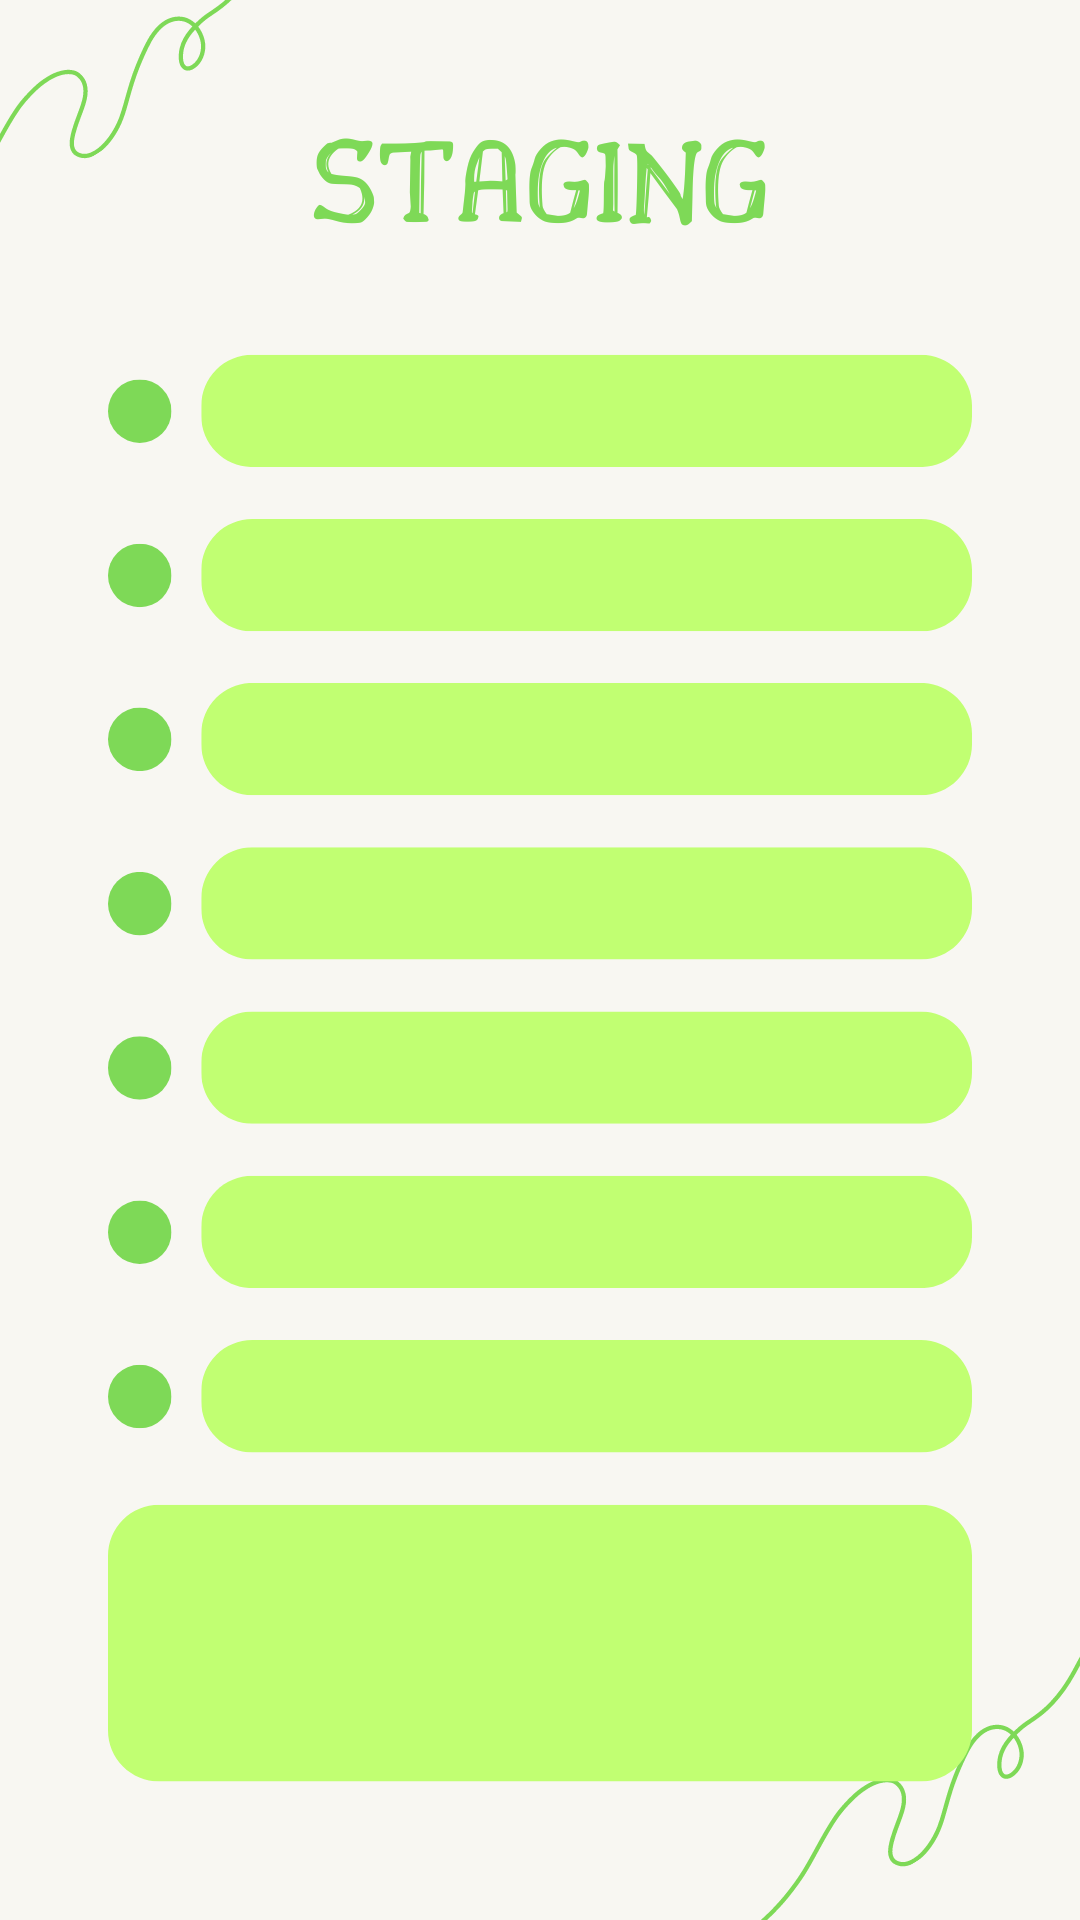
\includegraphics[width=\textwidth]{pictures/STAGING.png}
% https://www.canva.com/design/DAGDrwKlKDU/5tBfEI7Mzsp5s6nIUIs7Tw/edit?utm_content=DAGDrwKlKDU&utm_campaign=designshare&utm_medium=link2&utm_source=sharebutton
\end{column}

\begin{column}{0.24\textwidth}
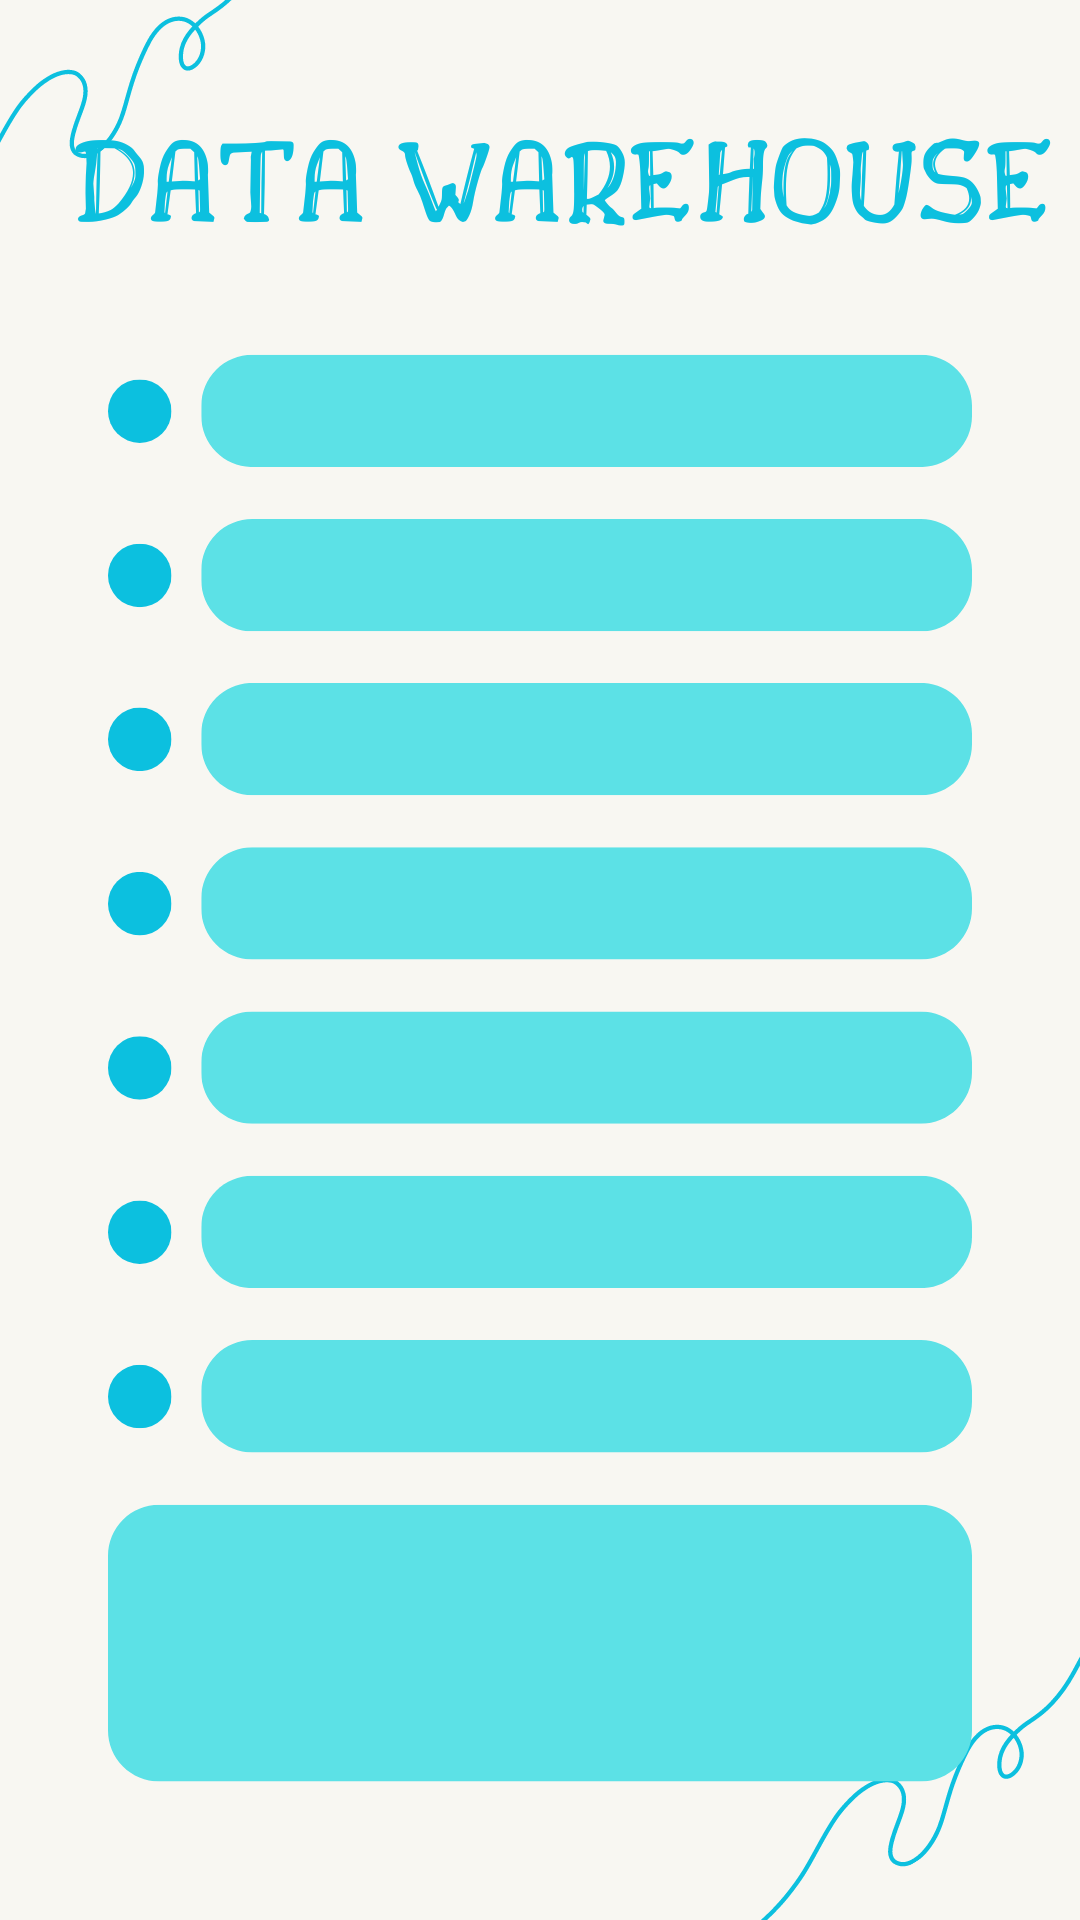
\includegraphics[width=\textwidth]{pictures/DATA WAREHOUSE.png}
% https://www.canva.com/design/DAGDr7K5Yq0/Z64jK07TlLNI0mGCIvUdrQ/edit?utm_content=DAGDr7K5Yq0&utm_campaign=designshare&utm_medium=link2&utm_source=sharebutton
\end{column}

\begin{column}{0.24\textwidth}
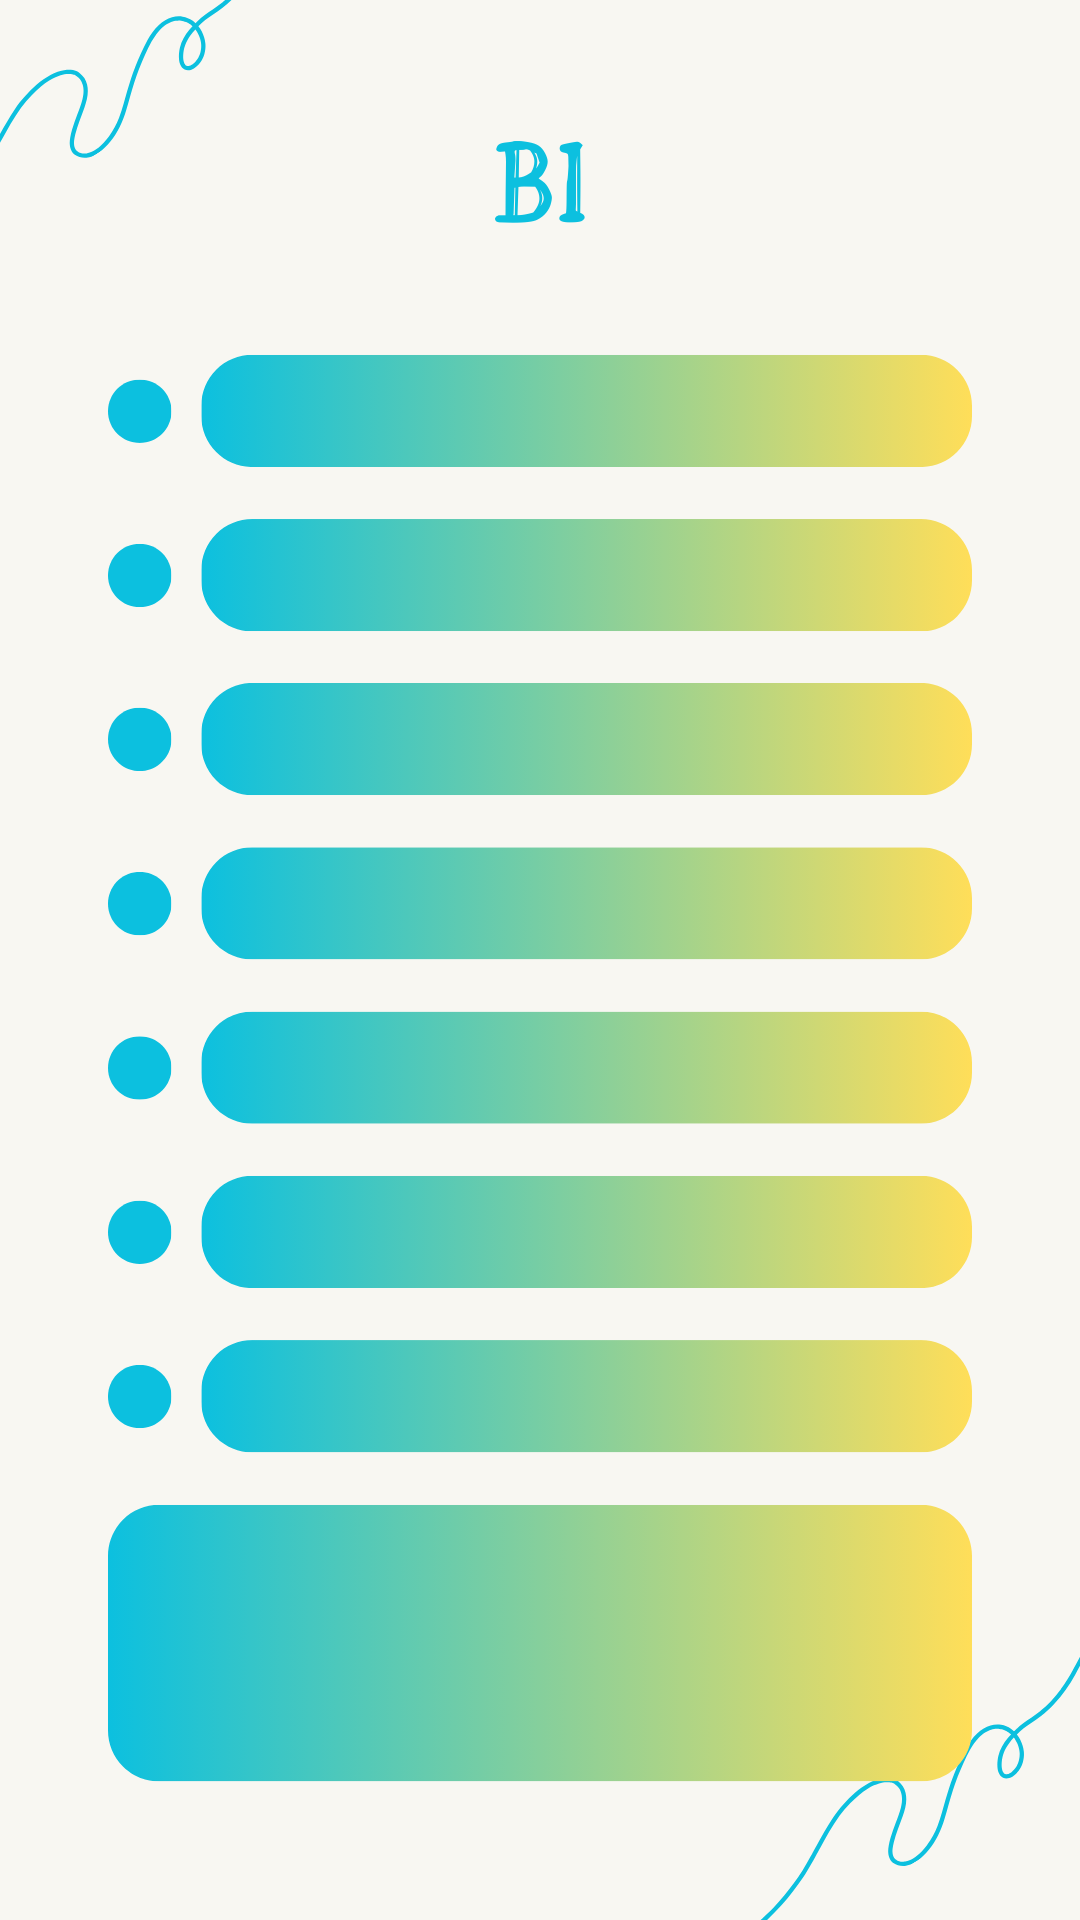
\includegraphics[width=\textwidth]{pictures/BI.png}
% https://www.canva.com/design/DAGDrwE3P6s/0GVeEFesokKj0oLIIrbjhg/edit?utm_content=DAGDrwE3P6s&utm_campaign=designshare&utm_medium=link2&utm_source=sharebutton
\end{column}

\end{columns}
\end{frame}
%%%%%%%%%%%%%%%%%%%%%%%%%%%%%%%%%%%%%%%%%%%%%%%%%%%%%%%

%! %%%%%%%%%%%%%%%%%%%%%%%%%%%%%%%%%%%%%%%%%%%%%%%%%%%%%%
\end{document}
%! %%%%%%%%%%%%%%%%%%%%%%%%%%%%%%%%%%%%%%%%%%%%%%%%%%%%%%

\subsection{ETL}
\begin{frame}{ETL}

\begin{columns}

\begin{column}{0.49\textwidth}
\begin{center}
\textcolor{red}{BEFORE}
%

\includegraphics[scale = 0.2]{pictures/black.png}
\end{center}
\end{column}

\begin{column}{.02\textwidth}
\rule{.1mm}{0.7\textheight}
\end{column}

\begin{column}{0.49\textwidth}
\begin{center}
\textcolor{red}{AFTER}
%

\includegraphics[scale = 0.2]{pictures/black.png}
\end{center}
\end{column}
\end{columns}

\end{frame}
%%%%%%%%%%%%%%%%%%%%%%%%%%%%%%%%%%%%%%%%%%%%%%%%%%%%%%%
\subsection{ETL}
\begin{frame}{ETL}

\begin{columns}

\begin{column}{0.49\textwidth}
\begin{center}
\textcolor{red}{BEFORE}
%

\includegraphics[scale = 0.2]{pictures/black.png}
\end{center}
\end{column}

\begin{column}{.02\textwidth}
\rule{.1mm}{0.7\textheight}
\end{column}

\begin{column}{0.49\textwidth}
\begin{center}
\textcolor{red}{AFTER}
%

\includegraphics[scale = 0.2]{pictures/black.png}
\end{center}
\end{column}
\end{columns}

\end{frame}
%! %%%%%%%%%%%%%%%%%%%%%%%%%%%%%%%%%%%%%%%%%%%%%%%%%%%%%%
%! %%%%%%%%%%%%%%%%%%%%%%%%%%%%%%%%%%%%%%%%%%%%%%%%%%%%%%
%! %%%%%%%%%%%%%%%%%%%%%%%%%%%%%%%%%%%%%%%%%%%%%%%%%%%%%%
%! %%%%%%%%%%%%%%%%%%%%%%%%%%%%%%%%%%%%%%%%%%%%%%%%%%%%%%
%! %%%%%%%%%%%%%%%%%%%%%%%%%%%%%%%%%%%%%%%%%%%%%%%%%%%%%%
\section{Xây dựng Dashboard}
\begin{frame}{xxxxxxxxxxxxx}
\begin{itemize}
\item Nội dung xxxxxxxxxxxxx
\end{itemize}
\end{frame}
%%%%%%%%%%%%%%%%%%%%%%%%%%%%%%%%%%%%%%%%%%%%%%%%%%%%%%%
\subsection{Mã QR Dashboard}
\begin{frame}{Mã QR Dashboard}

\begin{figure}[H]
\centering

\includegraphics[scale = 0.15]{pictures/black.png}
\end{figure}

\end{frame}
%! %%%%%%%%%%%%%%%%%%%%%%%%%%%%%%%%%%%%%%%%%%%%%%%%%%%%%%
%! %%%%%%%%%%%%%%%%%%%%%%%%%%%%%%%%%%%%%%%%%%%%%%%%%%%%%%
%! %%%%%%%%%%%%%%%%%%%%%%%%%%%%%%%%%%%%%%%%%%%%%%%%%%%%%%
%! %%%%%%%%%%%%%%%%%%%%%%%%%%%%%%%%%%%%%%%%%%%%%%%%%%%%%%
%! %%%%%%%%%%%%%%%%%%%%%%%%%%%%%%%%%%%%%%%%%%%%%%%%%%%%%%
\section{Tổng kết}
\begin{frame}{xxxxxxxxxxxxx}
\begin{itemize}
\item Nội dung xxxxxxxxxxxxx
\end{itemize}
\end{frame}
%%%%%%%%%%%%%%%%%%%%%%%%%%%%%%%%%%%%%%%%%%%%%%%%%%%%%%%

%%%%%%%%%%%%%%%%%%%%%%%%%%%%%%%%%%%%%%%%%%%%%%%%%%%%%%%
%%%%%%%%%%%%%%%%%%%%%%%%%%%%%%%%%%%%%%%%%%%%%%%%%%%%%%%
%%%%%%%%%%%%%%%%%%%%%%%%%%%%%%%%%%%%%%%%%%%%%%%%%%%%%%%
%%%%%%%%%%%%%%%%%%%%%%%%%%%%%%%%%%%%%%%%%%%%%%%%%%%%%%%
%%%%%%%%%%%%%%%%%%%%%%%%%%%%%%%%%%%%%%%%%%%%%%%%%%%%%%%
\section*{}
\begin{frame}{}
\centering
\Huge{Thanks for listening!}
\end{frame}
%%%%%%%%%%%%%%%%%%%%%%%%%%%%%%%%%%%%%%%%%%%%%%%%%%%%%%%
\end{document}
%%%%%%%%%%%%%%%%%%%%%%%%%%%%%%%%%%%%%%%%%%%%%%%%%%%%%%%

%%%%%%%%%%%%%%%%%%%%%%%%%%%%%%%%%%%%%%%%%%%%%%%%%%%%%%%

https://www.kaggle.com/code/colara/human-resources-analytics-a-descriptive-analysis
https://www.kaggle.com/datasets/rishikeshkonapure/hr-analytics-prediction
https://www.kaggle.com/code/jacksonchou/hr-analytics
https://www.kaggle.com/datasets/davidepolizzi/hr-data-set-based-on-human-resources-data-set
https://www.kaggle.com/datasets/rhuebner/human-resources-data-set
https://www.kaggle.com/code/sayamkumar/employee-attrition-prediction/input

https://www.kaggle.com/docs/api
https://www.kaggle.com/datasets/rhuebner/human-resources-data-set/data
https://www.kaggle.com/datasets/sherrytp/airline-delay-analysis?fbclid=IwAR2wsZkBGKgSIZj29PQLxTqLvoqG9HuLFjCWxrKztTzGRuGAOG5EiqqhvVg

https://downloadlynet.ir/2024/28/116039/01/machine-learning-data-science-with-python-kaggle-pandas/20/?#/116039-udemy-182411021524.html
https://downloadlynet.ir/2024/28/116043/01/machine-learning-data-science-with-python-kaggle-a-z/21/?#/116043-udemy-182411020524.html
%%%%%%%%%%%%%%%%%%%%%%%%%%%%%%%%%%%%%%%%%%%%%%%%%%%%%%%